\documentclass[twoside]{article}
\usepackage{aistats2016}
%\usepackage[accepted]{aistats2016}

\usepackage{amssymb,amsmath,natbib,graphicx,amsthm,
  setspace,sectsty,anysize,times,dsfont,enumerate}

\usepackage[svgnames]{xcolor}

\usepackage{lscape,arydshln,relsize,rotating,multirow}
\usepackage{algorithm,algorithmic}


\newtheorem{prop}{\sc Proposition}[section]
\newtheorem{theorem}{\sc Theorem}[section]
\newtheorem{definition}{\sc Definition}[section]
\newtheorem{lemma}{\sc Lemma}[section]
\newtheorem{corollary}{\sc Corollary}[section]
\DeclareMathOperator*{\argmin}{argmin}

\marginsize{1.1in}{.9in}{.3in}{1.4in}

\newcommand{\nb}{\color{blue}}
\newcommand{\dbl}{\setstretch{1.5}}
\newcommand{\sgl}{\setstretch{1.2}}

\newcommand{\bs}[1]{\boldsymbol{#1}}
\newcommand{\mc}[1]{\mathcal{#1}}
\newcommand{\mr}[1]{\mathrm{#1}}
\newcommand{\bm}[1]{\mathbf{#1}}
\newcommand{\ds}[1]{\mathds{#1}}
\newcommand{\indep}{\perp\!\!\!\perp}


\begin{document}

\twocolumn[

\aistatstitle{One-step estimator paths for concave regularization}

\aistatsauthor{ Matt Taddy }

\aistatsaddress{The  University of Chicago Booth School of Business} ]

\begin{abstract}
The statistics literature of the past 15 years has established many favorable
 properties for sparse diminishing-bias regularization: techniques which can
 roughly be understood as providing estimation under penalty functions
 spanning the range of concavity between $L_0$ and $L_1$ norms.  However,
 lasso $L_1$-regularized estimation remains the standard tool for industrial
 `Big Data' applications because of its minimal computational cost and the
 presence of easy-to-apply rules for penalty selection.   In response, this
 article proposes a simple new algorithm framework that requires no more
 computation than a lasso path: the path of one-step estimators (POSE) does
 $L_1$ penalized regression estimation on a grid of decreasing penalties, but
 adapts coefficient-specific weights to decrease as a function of the
 coefficient estimated in the previous path step.  This provides sparse
 diminishing-bias regularization at no extra cost over the fastest lasso
 algorithms. Moreover, our `gamma lasso' implementation of POSE is accompanied
 by a reliable heuristic for the fit degrees of freedom, so that
 standard information criteria can be applied in penalty selection. The
 methods are illustrated in extensive simulations and in application of
 logistic regression to evaluating the performance of hockey players.
 \end{abstract}

\section{Introduction}
\label{intro}

For regression in high-dimensions, it is useful to regularize estimation
through a penalty on coefficient size.   $L_1$  regularization \citep[i.e.,
the lasso of][]{tibshirani_regression_1996} is especially popular, with costs
that are non-differentiable at their minima and can lead to  coefficient
solutions of exactly zero.  A related approach is concave penalized
regularization (e.g. SCAD from \citealt{fan_variable_2001} or MCP from
\citealt{zhang_nearly_2010}) with cost functions that are also spiked at zero
but flatten for large values (as opposed to the constant increase of an $L_1$
norm).  This yields sparse solutions where  large non-zero values are estimated
with little bias. 

The combination of  \textit{sparsity} and \textit{diminishing-bias} 
 is appealing in many settings, and a large literature on concave
penalized estimation has developed over the past 15 years.  For example, many
authors (e.g., from \citealt{fan_variable_2001} and
\citealt{fan_nonconcave_2004})  have contributed work on their \textit{oracle
properties}, a class of results showing conditions under which coefficient
estimates through concave penalization, or in related schemes, will be the
same as if you knew the sparse `truth' (either asymptotically or with high
probability).   From an information compression perspective,  the increased
sparsity encouraged by diminishing-bias penalties (since single large
coefficients are allowed to account for the signals of other correlated
covariates) leads to lower memory, storage, and communication requirements.
Such savings are very important in distributed  computing schemes
\citep[e.g.,][]{taddy_distributed_2013}.



Unfortunately,  exact solvers for concave penalized estimation  all require
significantly more compute time than a standard lasso.  In our experience,
this has precluded their use in settings -- e.g., in text or web-data analysis
-- where both $n$ (the number of observations) and $p$ (the number of
   covariates) are very large. As we review below,  recent literature
   recommends the use of approximate solvers. Certainly, this is necessary for
   data of the size we encounter in analysis of, say, internet commerce.
   These approximations  take the form of iteratively-weighted-$L_1$
   regularization, where the coefficient-specific weights are based upon
   estimates of the coefficients taken from previous iterations of the
   approximate solver.  This literature
\citep[e.g.,][]{zou_one-step_2008,fan_strong_2014} 
holds that even a single step of weighted-$L_1$ regularization is enough to
get solutions that are close to optimal, so long as the pre-estimates are
\textit{good enough} starting points. The crux of success with such one-step
estimation (OSE) is  finding starts that are, indeed, good enough.


This article provides a complete framework for sparse diminishing-bias
regularization that combines ideas from OSE with the concept of a
\textit{regularization path} -- a general technique, most famously associated
with the LARS algorithm \cite{efron_least_2004}, that estimates a sequence of
models under decreasing amounts of regularization.  So long as the model estimates do not change too much from one level of regularization to the next, such path algorithms can be very fast to run and are an efficient way to obtain a high-quality \textit{set} of models to choose amongst.  

A path of one-step estimators (POSE; detailed in Section \ref{pose})
algorithm does $L_1$ penalized regression estimation on a grid of decreasing
penalties, but adapts coefficient-specific weights to decrease as a function
of the coefficient estimated in the previous path step.  POSE takes advantage
of the natural match between path algorithms and one-step estimation: OSE
relies upon inputs being close to the optimal solution, which is precisely the
setting where path algorithms are most efficient.  This framework 

The later penalty-selection capability is derived from a Bayesian interpretation for our \textit{gamma lasso} implementation of POSE (Section , from which we are able to derive heuristic information criteria 

We view such penalty-selection tools as an essential ingredient for practical applicability in large-scale industrial machine learning, where, e.g., cross-validation is not always viable or advisable.


\section{Path of one-step estimators}
\label{pose}

Our path of one-step estimators (POSE), in Algorithm \ref{posealgo}, uses solutions along the sequence of decreasing penalty sizes, $\lambda^t$, as the basis for LLA weights at the next path step.  In this, we are assuming a penalty specification such that $\lim_{b\to 0} c'(|b|) = 1$ and that the cost function is differentiable for $b\neq 0$.  This yields a path of one-step LLA
penalized coefficient estimates. 

\vskip .2cm
{
\begin{algorithm}[ht]
\caption{\label{posealgo} POSE }
\vskip .2cm
Initialize $\bs{\hat\beta}^0 = \bf{0}$, so that $\hat S_0 = \varnothing$.

\vskip .2cm
Set $\lambda^1 >
0$ with step size
$0 < \delta < 1$.

\vspace{-.75cm}
\begin{align}
\text{for}~t=1\ldots T :&\notag \\
\omega^{t}_j  &=  
\left\{ 
  \begin{array}{r}
    c'(|\hat\beta^{t-1}_j|) ~\text{for}~j \in \hat S_t \\
    1  ~\text{for}~j \in \hat S_t^c  
  \end{array} 
  \right. 
  \label{wset}\\
\left[\hat\alpha,\bs{\hat\beta}\right]^t &= \argmin_{\alpha,\beta_j\in\ds{R}}~~
l(\alpha,\bs{\beta}) + n\sum_j \lambda^t\omega^t_j|\beta_j| \label{l1pen}\\
\lambda^{t+1} &= \delta \lambda^t\notag
\end{align}
\vskip -.3cm
\end{algorithm}}

 From an engineering standpoint, POSE has the same appeal as any successful path algorithm: if the estimates change little from iteration $t$ to $t+1$, then you will be able to quickly solve for a large set of candidate specifications.  Following the discussion of Section \ref{rp}.1, such algorithms are a natural match with one-step estimation: OSE relies upon inputs being close to the optimal solution, which is precisely the setting where path algorithms are most efficient.  More rigorously, Theorem \ref{sparseapprox} applied to POSE yields  $\hat S_{t-1} \cap S^c = \varnothing \Rightarrow \omega_{S^c}^{t~\mr{min}} = 1$.  Thus so long as $\lambda$ is large enough,  Section \ref{rp}.2 demonstrates that  fast diminishing $\omega_j$ will help control false discovery and improve prediction.  Of course, the moment $\hat S_t \cap S^c \neq \varnothing$,  diminishing-bias allows spurious covariates to enter with  little shrinkage and can move the fit arbitrarily far away from $L_0$-optimality -- that is, with $\lambda$ too small the diminishing bias hurts your ability to estimate and predict.  This is why it is essential to have a path of candidate $\lambda^t$ to choose amongst.


\section{Sparse regularization paths and diminishing bias}
\label{rp}




\section{The gamma lasso}
\label{sec:gamlr}

The gamma lasso (GL) specification for POSE is based upon the log penalty,
\begin{equation}\label{logpen}
c(\beta_j) =  \log(1+\gamma|\beta_j|),
\end{equation} where $\gamma > 0$.  This
penalty is concave with curvature $-1/(\gamma^{-1}+|\beta_j|)^2$ and it spans the
range from $L_0$ ($\gamma\rightarrow \infty$) to $L_1$ ($\gamma\rightarrow 0$)
costs (see Figure \ref{solution}).  It appears under a variety of parameterizations and names in the
literature; see
\citet{mazumder_sparsenet_2011} and applications in
\citet{friedman_fast_2008}, \citet{candes_enhancing_2008},
\citet{cevher_learning_2009}, \citet{taddy_multinomial_2013} and \citet{armagan_generalized_2013}. 

GL -- POSE under the log penalty  -- leads to line (\ref{wset}) being replaced by
\begin{equation}\label{gammalasso}
\omega^{t}_j  = \left(1 + \gamma |\hat\beta^{t-1}_j|\right)^{-1} ~~j=1\ldots p 
\end{equation}
Behavior of the resulting paths  is governed by $\gamma$, which we refer to as the
penalty {\it scale}.  Under $\gamma=0$, GL is just the usual lasso.
 Bias diminishes faster for larger $\gamma$ and, at the  extreme,
$\gamma=\infty$ yields a subset selection routine where a coefficient is
unpenalized in all segments after it first becomes nonzero. Figure
\ref{gamlr_eg} shows solutions in a simple problem.


\begin{figure}[t]
\hskip -.2cm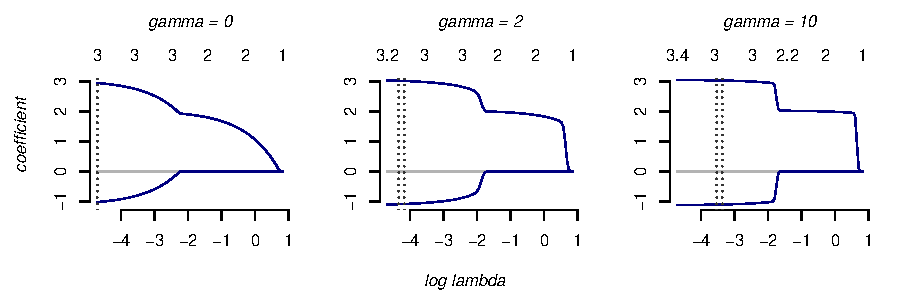
\includegraphics[width=6.5in]{gamlr_eg}
\vskip -.25cm
\caption{\label{gamlr_eg} Gamma lasso estimation on $n=10^3$ 
 observations of $y_i = 4 + 3x_{1i} - x_{2i} + \varepsilon_i$, where
$\varepsilon_i \stackrel{ind}{\sim} \mr{N}(0,1)$ and
$\{x_{1i},x_{2i},x_{3i}\}$ are marginally standard normal with correlation of
0.9 between covariates ($x_{3i}$ is spurious). The penalty path has $T=100$
segments, $\lambda^1 = n^{-1}\left| \sum_i x_{1i}y_i\right|$, and
$\lambda^{100} = 0.01\lambda^1$. Degrees of freedom are on top and vertical
lines mark AICc and BIC selected models (see Section
\ref{sss}).}
\vskip -.25cm
\end{figure}

Each  gamma lasso path segment is solved through coordinate descent,
as detailed in Appendix \ref{implement}.  The algorithm is implemented in {\tt
c} as part of the {\tt gamlr} package for {\sf R}. The software  has detailed documentation and versioned source code is at
{\tt github.com/mataddy/gamlr}.  Usage of {\tt gamlr} mirrors that of its
convex penalty analogue {\tt glmnet} \citep{friedman_regularization_2010}, the
fantastic and widely used package for costs between $L_1$ and $L_2$ norms. In
the lasso case ($\gamma=0$), the two algorithms are essentially equivalent.


\subsection{Bayesian motivation}

Consider a model where each $\beta_j$ is
assigned a Laplace distribution prior with scale $\tau_j>0$,
\begin{equation}\label{blasso}
\beta_j \sim \mr{La}\left(\tau_j\right) =
\frac{\tau_j}{2}\exp\left[ -\tau_j|\beta_j| ~\right].
\end{equation}
Typically, scale parameters $\tau_1 =
\ldots = \tau_p$ are set as a single shared value, say $n\lambda/\phi$ where
 $\phi$ is the exponential family dispersion (e.g. Gaussian variance
$\sigma^2$ or 1 for the binomial).   Posterior
maximization under the prior in (\ref{blasso}) is then lasso estimation \citep[e.g.,][]{park_bayesian_2008}.

Instead of working from shared scale, assume an independent gamma
$\mr{Ga}(s,1/\gamma)$ hyperprior with `shape' $s$ and `scale' $\gamma$ for
each $\tau_j$, such that $\ds{E}[\tau_j] = s\gamma$ and $\mr{var}(\tau_j) =
s\gamma^2$.  Then the {\it joint} prior for both coefficient and scale is
\begin{equation}\label{glprior}
\pi(\beta_j,\tau_j) = \mr{La}\left(\beta_j ;~ \tau_j\right)
\mr{Ga}\left(\tau_j;~ s,\gamma^{-1}\right) = \frac{ 1}{2\Gamma({s})} 
\left(\frac{\tau_j}{\gamma}\right)^{s}
               \exp\left[-\tau_j(\gamma^{-1}+|\beta_j|)\right].
\end{equation}
The gamma hyperprior is conjugate here, implying a $\mr{Ga}\left(s+1, ~1/\gamma +
|\beta_j|\right)$ posterior for $\tau_j \mid \beta_j$ with conditional
posterior mode (MAP) at $\hat\tau_j = \gamma s/(1 + \gamma |\beta_j|)$.

Consider joint MAP estimation of $[\bs{\tau},\bs{\beta}]$ under the prior in
   (\ref{glprior}), where we've suppressed $\alpha$ for simplicity. By taking
   negative logs and removing constants, this is equivalent to solving
\begin{equation}\label{gljoint}
\min_{\beta_j\in\ds{R},~\tau_j \in \ds{R}^{+}}~~
\phi^{-1}l(\bs{\beta}) + \sum_j \left[\tau_j(\gamma^{-1}+|\beta_j|) - s\log(\tau_j)\right].
\end{equation}
It is straightforward to show that (\ref{gljoint}) is equivalent 
to the log-penalized objective 
\begin{equation}\label{logobj}
\min_{\beta_j\in\ds{R}}~~
\phi^{-1}l(\bs{\beta}) + \sum_j  s\log(1+\gamma|\beta_j|)
\end{equation}

\begin{prop}\label{penprop}
  $\bs{\hat\beta}$ solves (\ref{logobj}) if and only if it is also in the
  solution to (\ref{gljoint}).
\end{prop}
\begin{proof}
  The conditional posterior mode for each $\tau_j$ given $\beta_j$
  is $\tau(\beta_j) = \gamma s/(1 + \gamma|\beta_j|)$.  Any joint solution
  $[\bs{\hat\beta},\bs{\hat\tau}]$ for (\ref{gljoint}) thus
  consists of $\hat{\tau}_{j} = \tau(\hat\beta_{j})$;
  otherwise, it is always possible to decrease the objective by
  replacing $\hat\tau_{j}$. Setting each $\tau_j = 
  \tau(\beta_j)$ in (\ref{gljoint}) and removing constant terms yields
  (\ref{logobj}).  Moreover, the solution to (\ref{gljoint}) solves
  (\ref{logobj}): otherwise, there would need to be a point on the profile
  slice of (\ref{gljoint}) defined by $\tau_{j} =
  \tau(\hat\beta_{j})$ that is lower than its minimum.
\end{proof}

For a Bayesian it is odd to be solving for $\bs{\tau}$ rather than
marginalizing over its uncertainty.  However, recognizing the form of a gamma
density  in (\ref{glprior}), $\pi(\beta_j,\tau_j)$ integrates over $\tau_j$ to
yield the marginal prior $ \pi(\beta_j) = 0.5s\left( 1+
\gamma|\beta_j|\right)^{-(s+1)}$. This is the generalized double Pareto
density, as in  \citet{armagan_generalized_2013}. Since $-\log \pi(\beta_j)
\propto (s+1)\log(1 + \gamma|\beta_j|)$, the {\it profile} MAP solution to
(\ref{gljoint}) is also the {\it marginal} MAP for
$\bs{\beta}$ under $\mr{Ga}(s-1,1/\gamma)$ priors on each $\tau_j$.


\setstretch{1}
\bibliographystyle{chicago}
\bibliography{pose}

\end{document}
